\documentclass[preprint,12pt]{elsarticle}
\usepackage{amsmath,amssymb,bm}
\usepackage{booktabs,multirow,threeparttable}
\usepackage{graphicx,subcaption}
\usepackage{xcolor,hyperref,lineno,enumitem,microtype,placeins}
\emergencystretch=2em
\graphicspath{{../figures/}}
\hypersetup{colorlinks=true,linkcolor=blue!50!black,citecolor=blue!50!black,urlcolor=blue!60!black}
\journal{Transportation Research Part C}
\newcommand{\IJS}{\mathrm{IJS}}

\begin{document}
\begin{frontmatter}

\title{Data-driven collaborative optimization of three-dimensional highway alignments for life-cycle cost and mixed fuel--electric traffic energy}

\author[aff1]{Anonymous Author(s)}
\affiliation[aff1]{organization={Anonymous institution for double-anonymized review},
  city={Anonymous}, country={China}}

\begin{abstract}
Horizontal and vertical highway alignment decisions jointly determine terrain disturbance, structures, construction expenditure and long-term vehicle operation. This study develops a spatially explicit bi-objective framework that combines 14,018 GNSS centerline points, a quasi-natural digital elevation model reconstructed after masking the existing roadway, and OpenStreetMap transport and water features. Candidate plans are represented by 50 sine modes, whereas one start-elevation variable and 224 segment grades describe the profile. Life-cycle cost covers land, basic works, structures, earthwork and maintenance; the second objective monetizes 30-year fuel and electricity use for a mixed fleet. Intersections with qualifying OSM features trigger bridge intervals, a connected mountain zone triggers ecological tunnelling, and Improved Jellyfish Search (IJS) approximates the cost--energy front. Feasibility, a planning budget, non-dominance and entropy weighting are applied sequentially to select a compromise.

For the 22.46-km Guangzhou North Ring case, the feasible joint solution reduces cost from 2.6406 to 2.4224 billion RMB (8.26\%) and monetized energy from 1.3946 to 1.3477 billion RMB (3.37\%). It shortens the line by 98.3 m and satisfies the 400-m radius requirement with $R_{min}=401.0$ m and zero stored penalty. Structure cost decreases by 261.4 million RMB, offsetting a 45.5-million-RMB earthwork increase. A sequential solution has lower raw objectives but is infeasible ($R_{min}=397.1$ m). Same-generation ablation and algorithm tests show the lowest observed mean objective for IJS, although unequal function-evaluation counts preclude an equal-budget superiority claim. The unanchored vertical endpoints and single-direction energy calculation limit the result to corridor-planning evidence.
\end{abstract}

\begin{keyword}
highway alignment optimization \sep digital elevation model \sep OpenStreetMap \sep improved Jellyfish Search \sep life-cycle cost \sep traffic energy \sep horizontal--vertical coordination
\end{keyword}
\end{frontmatter}

\linenumbers

\section{Introduction}

Highway alignment is an early decision with long-lived consequences. A lateral shift changes the terrain crossed, land occupation, bridge and tunnel demand, earthwork balance and grades experienced by vehicles. These effects are coupled: a shorter plan may worsen the profile, avoiding a mountain may create additional crossings, and a locally cheap profile may become geometrically infeasible. Alignment selection is therefore a constrained spatial and multi-objective problem rather than separate curve fitting in plan and profile.

Classical formulations established the value of simultaneous horizontal and vertical optimization \cite{chew1989,jong2003}. Later work introduced GIS corridors, mixed-integer models, environmental objectives and preference-aware search \cite{kang2012,mondal2015,hirpa2016,vazquez2018,akhmet2022}. Recent studies combine alignment generation with BIM, reinforcement learning, sampling-based planning and hybrid metaheuristics \cite{han2023,he2023,alhadad2024,pu2024,pu2026}. Nevertheless, heterogeneous spatial data and traceable engineering accounting remain difficult to integrate consistently \cite{songreview2023}.

Three gaps motivate this study. First, a single centerline terrain profile cannot reflect the terrain encountered after horizontal displacement. Second, fixed bridge and tunnel allowances may allow the optimizer to exploit accounting assumptions instead of locating a constructible corridor. Third, high-dimensional plan--profile search needs both global exploration and local refinement, while feasibility must be checked at fine spatial resolution.

This paper contributes:

\begin{enumerate}[leftmargin=*,label=(\arabic*)]
\item a digital corridor linking each candidate plan to a quasi-natural DEM and OSM crossing features;
\item an auditable life-cycle formulation with geometry-triggered bridges, ecological tunnelling and earthwork-to-structure substitution;
\item a 275-variable collaborative plan--profile representation and a cost--energy decision sequence that places feasibility before entropy weighting; and
\item a boundary-aware evaluation of IJS, including the engineering solution, a joint-versus-sequential control, same-generation mechanism ablation, multi-algorithm tests and re-optimization sensitivity analysis.
\end{enumerate}

Figure~\ref{fig:overview} summarizes the workflow. All numerical claims in this manuscript are fixed to repository commit \texttt{c1327df}; no later endpoint or density formulation is mixed into the evidence. The full hash is recorded in the accompanying source manifest.

\begin{figure}[!htbp]
\centering
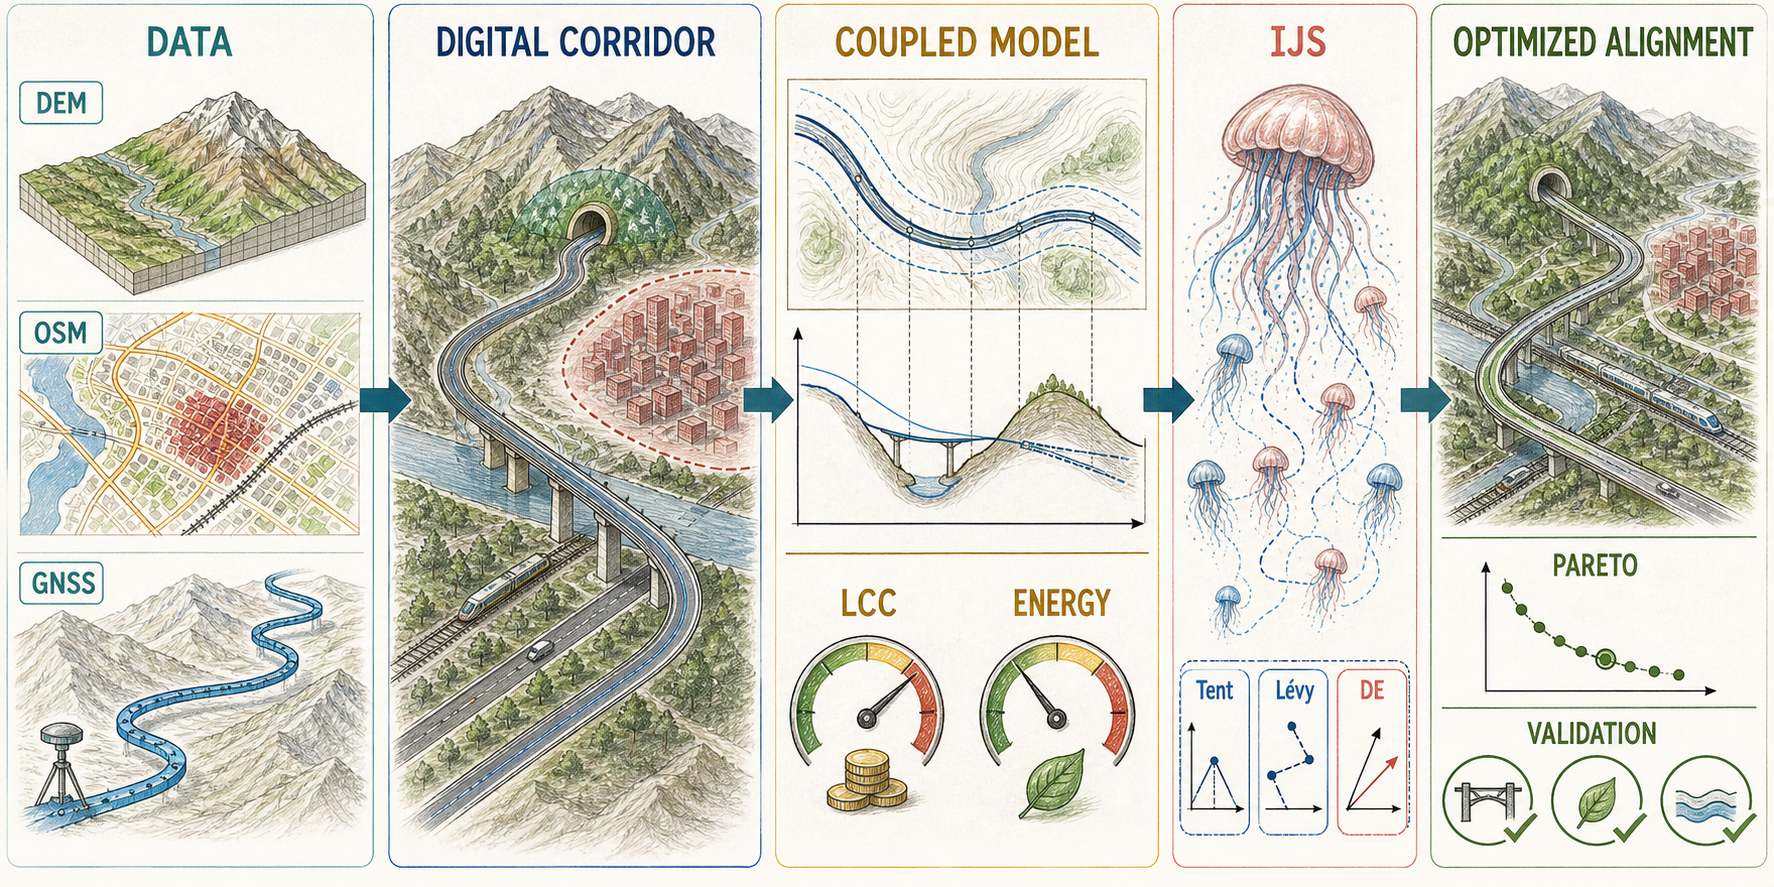
\includegraphics[width=\textwidth]{method_overview_handdrawn.png}
\caption{Data-driven workflow from spatial data and coupled objectives to IJS search and compromise selection. Buildings in the illustration provide corridor context; the pinned model uses DEM and OSM transport/water crossings but contains no building-density constraint.}
\label{fig:overview}
\end{figure}

\section{Related research}

\subsection{Three-dimensional alignment optimization}

Simultaneous plan--profile models avoid inconsistencies caused by sequential design \cite{chew1989,jong2003}. GIS-based methods broadened the feasible corridor and incorporated environmental layers \cite{kang2012,davey2017}; corridor-constrained and mathematical-programming approaches improved tractability \cite{mondal2015,akhmet2022}. Bi-objective highway and railway models further introduced cost, hazard and ecological performance \cite{hirpa2016,zhang2020,song2022}. The present study emphasizes a traceable mapping from candidate coordinates to terrain, crossings, quantities and objectives.

\subsection{Life-cycle cost and traffic energy}

The cost categories follow the mathematical base in Lin \cite{lin2025}: land, bridge/tunnel works, basic works, maintenance and earthwork. Road geometry affects vehicle energy through distance, grade and curvature \cite{llopis2019}; electric-vehicle consumption also depends on drivetrain efficiency and regenerative operation \cite{dimartino2022}. Fuel and electricity are therefore retained separately and then monetized over a common 30-year horizon. Monetary aggregation provides a decision scale but is not a complete environmental assessment.

\subsection{Search and compromise selection}

NSGA-II is a standard multi-objective benchmark \cite{deb2002}. Jellyfish Search (JS) alternates ocean-current and active/passive movement \cite{chou2021}. The implemented IJS adds Tent initialization, L\'evy exploration and differential-evolution (DE) refinement \cite{storn1997}. Entropy weighting, derived from Shannon information \cite{shannon1948}, is used twice: first to establish a common scalar search direction and later to select among feasible non-dominated candidates. The two uses are kept distinct.

\section{Data-driven mathematical formulation}\label{sec:model}

\subsection{Study corridor and spatial data}

The case covers the Xunfengzhou--Huangcun section of Guangzhou North Ring Expressway, a two-way six-lane urban expressway. The measured M-A centerline contains 14,018 GNSS points and is 22.4618 km long under the common evaluator. All candidates share the measured plan endpoints.

Terrain is obtained from 60 AWS Terrain Tiles at zoom level 14, approximately 8.8 m per pixel \cite{awsterrain}. To reduce the influence of the built road surface, a $\pm60$-m mask around the existing road is removed and interpolated from adjacent terrain, producing a quasi-natural DEM. After a constant vertical-datum adjustment, the reconstructed surface has a correlation of 0.915 with measured centerline elevation. OSM supplies road, railway and water features \cite{haklay2008,osmlicense}. After removal of the North Ring Expressway and parallel facilities, the stored obstacle layer contains 4,807 road, 857 railway and 338 river/canal features.

The DEM is queried at the actual coordinates of each candidate line. Intersections with motorway, trunk or primary roads, railways and watercourses trigger bridge intervals. A connected high-terrain region represents the Baiyun ecological tunnel zone. OSM buildings are available only as visual context in this pinned version and do not enter the objective or constraints.

\subsection{Collaborative decision variables}

Let the measured plan be $\bm r_0(s)=[x_0(s),y_0(s)]^\top$ with unit normal $\bm n(s)$, $s\in[0,L_0]$. A candidate normal offset is
\begin{equation}
\delta(s)=\sum_{k=1}^{50}a_k\sin\left(\frac{k\pi s}{L_0}\right),
\qquad |a_k|\leq \frac{W}{k^2},
\label{eq:sine}
\end{equation}
and $\bm r(s)=\bm r_0(s)+\delta(s)\bm n(s)$. The sine basis fixes both plan endpoints and attenuates high-frequency curvature. In the main run $W=500$ m is the amplitude of the first mode, not a pointwise corridor half-width; the conservative envelope is $|\delta|\leq W\sum_{k=1}^{50}k^{-2}\approx1.625W$. Cubic-spline reconstruction is evaluated at approximately 10-m spacing. Curvature and radius are
\begin{equation}
\kappa(s)=\frac{|x'(s)y''(s)-y'(s)x''(s)|}
{[x'(s)^2+y'(s)^2]^{3/2}},\qquad R(s)=\kappa(s)^{-1}.
\label{eq:curvature}
\end{equation}

The profile block has $M=225$ normalized variables. With quasi-natural ground $z^g_0$, start-amplitude $A_0=20$ m, maximum grade $g_{max}=0.04$, control spacing $\Delta s_i$ and variables $u_i\in[0,1]$,
\begin{align}
z_0&=z^g_0+(2u_0-1)A_0,\\
g_i&=(2u_i-1)g_{max},\quad i=1,\ldots,224,\\
z_j&=z_0+\sum_{i=1}^{j}g_i\Delta s_i.
\label{eq:profile}
\end{align}
Thus the full search vector has 50 plan coefficients, one start-elevation variable and 224 grade variables, totaling 275 active variables. The grade bound is satisfied by construction. Crucially, Eq.~\eqref{eq:profile} does not anchor either profile endpoint to the measured road. The implication is reported explicitly in Section~\ref{sec:limitations}.

\subsection{Life-cycle cost}

The first objective is
\begin{equation}
\min C=C_R+C_B+C_S+C_Q+C_{TU},
\label{eq:lcc}
\end{equation}
where $C_R$, $C_B$, $C_S$, $C_Q$ and $C_{TU}$ denote land, bridge/tunnel, basic works, discounted maintenance and earthwork/haulage costs. With road width $B$, route length $L$, bridge and tunnel lengths $L_B,L_T$, and invariant interchange ramp cost $C_{ramp}$,
\begin{align}
C_R&=c_{land}\frac{LB}{666.67}+5000\frac{L}{1000},\\
C_B&=c_BL_B+C_{ramp}+c_TL_T,\\
C_S&=(c_{sg}+c_{pv})L,\label{eq:lccparts}\\
C_Q&=\sum_{y=1}^{T}\frac{1}{(1+r)^y}
\sum_i\Delta s_i[\gamma+365Q_y\tau+c_{soil}\Phi_i].
\end{align}
The analysis horizon is $T=30$ years and $r=5\%$. In the maintenance term, $\gamma=10$ RMB/m is the traffic-independent annual rate, $\tau=10^{-6}$ RMB/(vehicle-trip m) is the traffic coefficient, and $c_{soil}=2$ RMB/m weights slope exposure. Specifically, $\Phi_i=\alpha W_{s,i}m_s^2+\beta W_{h,i}m_h^2+(1-\alpha-\beta)(W_{s,i}m_s^2+W_{h,i}m_h^2)$, with $\alpha=\beta=0.3$. Here $W_{s,i}$ and $W_{h,i}$ are the cut- and fill-slope widths, and $m_s$ and $m_h$ are their side-slope ratios; both widths are zero on structure-exempt segments. Unit rates follow the source thesis and the Guangzhou governmental estimation guideline \cite{guangzhou2025}.

At station $j$, $h_j=z_j-z^g_j$ and the approximate earthwork area is
\begin{equation}
A_j=B|h_j|+m h_j^2.
\end{equation}
Cut and fill volumes use the average-end-area rule. For non-exempt stations, the code selects the lower of earthwork and the corresponding per-metre structure cost and forces structure substitution when $|h_j|>30$ m. The selected station rates are then integrated trapezoidally:
\begin{align}
V^{\pm}&=\sum_j\frac{A_j^{\pm}+A_{j+1}^{\pm}}{2}\Delta s_j,\\
c_j&=\begin{cases}
c_{str},& |h_j|>30~\mathrm{m}\ \text{or}\ c_{ew}A_j>c_{str},\\
c_{ew}A_j,&\text{otherwise},
\end{cases}\\
C_{TU}&=E_L+\sum_j\frac{c_j+c_{j+1}}{2}\Delta s_j.
\label{eq:earthwork}
\end{align}
Ecological-tunnel and crossing-bridge intervals are earthwork-exempt to prevent double counting. For an obstacle with nominal width $b_q$, crossing angle $\theta_q$ and approach extension $E_{ext}=75$ m, its bridge interval is
\begin{equation}
\ell_q=\frac{b_q}{\max(\sin\theta_q,\sin15^\circ)}+2E_{ext},
\end{equation}
and gaps below 100 m are merged.

\begin{table}[t]
\centering
\caption{Principal parameters of the pinned case model.}
\label{tab:parameters}
\resizebox{\linewidth}{!}{\begin{tabular}{lll}
\toprule
Group & Parameter & Value \\
\midrule
Geometry & speed / width / $R_{min}$ / $g_{max}$ & 100 km/h / 25.5 m / 400 m / 4\% \\
Representation & plan modes / profile variables / $W$ & 50 / 225 / 500 m \\
Life cycle & horizon / discount rate & 30 yr / 5\% \\
Structures & bridge / tunnel / $E_{ext}$ & 156 / 270 million RMB/km / 75 m \\
Earthwork & cut / fill / side slope & 30 / 25 RMB/m$^3$ / 1:1.5 \\
Traffic & AADT / EV share & 30,000 veh/day / 0.30 \\
Energy & fuel / electricity price & 8 RMB/L / 0.8 RMB/kWh \\
Search & population / iterations / weight points & 200 / 1,000 / 21 \\
\bottomrule
\end{tabular}}
\end{table}

\subsection{Mixed fuel--electric traffic energy}

The second objective is the discounted monetary cost of fuel and electricity:
\begin{equation}
\min E=\sum_{y=1}^{30}\frac{365Q_y}{(1+r)^y}
[(1-p_{EV})c_fe_f(\bm x)+p_{EV}c_ee_e(\bm x)].
\label{eq:energy}
\end{equation}
Here $e_f$ is single-vehicle single-trip fuel use in L and $e_e$ is electricity use in kWh. For a representative vehicle, aerodynamic, rolling, grade and residual lateral forces are
\begin{align}
F_{air}&=\tfrac12\rho C_dA_fv^2,&
F_r&=C_rm_vg\cos\vartheta,\\
F_g&=m_vg\sin\vartheta,&
F_a&=\max\left(0,\frac{m_vv^2/R-m_vgS_p}{N_vC_s}\right).
\end{align}
The grade angle is $\vartheta=\arctan g_i$. The implemented superelevation is $S_p=\min(S_{p,max},v^2/(gR))$, with $S_{p,max}=0.08$. The $10^{-3}$ multiplier printed at the end of the source-thesis lateral-force equation is omitted in the pinned implementation because it is dimensionally and numerically inconsistent; the equation above reports the committed implementation. Here $\rho=1.25$ kg/m$^3$, $C_d=0.28$, $A_f=2.0/2.2$ m$^2$, $C_r=0.015/0.012$, and $m_v=1500/1800$ kg for fuel/electric vehicles; $N_v=4$ and $C_s=43$. In Eq.~\eqref{eq:fuel}, $\phi=0.03$ ml/(s hp), $HP_{in}=27$ hp and $\eta_f=0.85$.
Fuel use converts positive external load to horsepower:
\begin{align}
P_{ex,i}&=\max\left(0,\frac{(F_{air}+F_r+F_g+F_a)v}{736\eta_f}\right),\\
e_f(\bm x)&=\sum_i\phi(HP_{in}+P_{ex,i})\frac{\Delta s_i}{v}/1000.
\label{eq:fuel}
\end{align}
For electric vehicles, with signed work $W_i=(F_{air}+F_r+F_g+F_a)\Delta s_i$,
\begin{equation}
e_e(\bm x)=\left[\frac{1}{3.6\times10^6}\sum_i
\begin{cases}W_i/\eta_e,&W_i\geq0,\\W_i\eta_e,&W_i<0,
\end{cases}\right]_+ +0.15L_{km},
\label{eq:ev}
\end{equation}
where $[x]_+=\max(x,0)$ and $\eta_e=0.90\times0.95$. The code evaluates one representative travel direction; fuel and electricity components remain separately reportable before aggregation.

\subsection{Constraints and decision rule}

The hard conditions in the pinned implementation are $R(s)\geq400$ m, $|g_i|\leq4\%$, adjacent grade-change limit $|g_{i+1}-g_i|\leq3\times10^{-4}\Delta s_{ctrl}$ and crossing skew angle $\theta\geq15^\circ$. Plan endpoints and grade bounds are satisfied by construction; vertical endpoints are free. Values follow JTG D20--2017 \cite{jtgd20} where directly applicable.

For a relative violation vector $\bm v$, define $H(\bm v)=\operatorname{mean}(\bm v)+\max(\bm v)$. With $v_R=[400-R]_+/400$, normalized grade-change excess $v_{\Delta g}$ and skew excess $v_{skew}$, the implemented penalty is
\begin{equation}
P=10\rho_t[H(\bm v_R)+H(\bm v_{\Delta g})+H(\bm v_{skew})],
\label{eq:penalty}
\end{equation}
where $\rho_t=0.3$ in the first search half and $3.0$ in the second. The mean-plus-maximum form prevents a short severe violation from being diluted by route length.

A common initial population supplies $C_{ref}$, $E_{ref}$ and entropy weights $(w_C,w_E)=(0.50838,0.49162)$. Each search minimizes
\begin{equation}
F(\bm x)=w_C\frac{C(\bm x)}{C_{ref}}+w_E\frac{E(\bm x)}{E_{ref}}+P(\bm x),
\label{eq:scalar}
\end{equation}
with $C_{ref}=4.04836$ billion RMB and $E_{ref}=1.40373$ billion RMB. Twenty-one values of $w_C\in[0,1]$ approximate the front. Candidates then pass four gates: $P\leq10^{-6}$, $C\leq1.1C_{M-A}$, non-dominance and entropy-weighted compromise selection. Front entropy gives $(0.41421,0.58579)$; the selected candidate originates from the $w_C=0.50838$ search.

\section{Improved Jellyfish Search}\label{sec:solver}

\subsection{Mechanisms}

The original JS alternates ocean-current motion toward the best solution with active/passive population movement \cite{chou2021}. The implemented IJS adds:

\begin{itemize}[leftmargin=*]
\item independent Tent-map initialization ($\mu=1.99$ in the actual algorithm);
\item L\'evy perturbations scaled by $0.01(\bm u-\bm l)$ for non-local exploration; and
\item DE mutation and crossover with $CR=0.5$, followed by elitist acceptance \cite{storn1997}.
\end{itemize}

At generation $t$, the JS time control is $A_r=(1-t/T)(2u-1)$. The implementation applies a JS trial, then a L\'evy trial and finally a DE trial, accepting improvements after each stage. Consequently a full IJS generation uses approximately three population-equivalent objective-evaluation phases, whereas plain JS uses one. The soft-to-hard penalty schedule is applied across two consecutive half-runs. Figure~\ref{fig:flow} summarizes the implemented process.

\begin{figure}[t]
\centering

\includegraphics[width=.72\linewidth]{ijs_flowchart_handdrawn.png}
\caption{IJS search and post-search decision sequence.}
\label{fig:flow}
\end{figure}

\subsection{Experimental design and statistical scope}

The engineering experiment uses $W=500$ m, 275 variables, population 200, 1,000 generations and 21 weight points. M-A is the existing line, M-B minimizes cost alone, and M-C is the final feasible entropy-selected joint solution. A two-stage control first minimizes plan-related life-cycle cost and freezes the resulting plan; the second stage then optimizes the profile using the joint experiment's common $C/E$ references and entropy weights. Each stage runs for 500 generations.

The mechanism ablation uses a measured-plan, 225-variable profile testbed with 30 independent runs, population 200 and 500 generations. The multi-algorithm test compares IJS, JS, NSGA-II, real-coded GA, PSO and GWO at six profile resolutions with ten runs per algorithm--resolution pair. Ablation $p$ values use the independent-sample Mann--Whitney U test, whereas benchmark $p$ values use the independent Wilcoxon rank-sum test (SciPy \texttt{ranksums}); neither analysis is paired. Because activating L\'evy and DE adds objective calls, equal generations do not imply equal numbers of function evaluations (NFE). These tests support observed same-generation differences, not equal-budget causal claims.

Sensitivity analysis contains 237 already-completed re-optimizations covering demand, fleet, energy prices, design parameters and spectral width. These data use the same free-endpoint model family as the pinned engineering result. No supplementary experiment is introduced in this manuscript.

\section{Results}

\subsection{Engineering result}

Table~\ref{tab:main} and Figure~\ref{fig:scheme} show the feasible joint solution. Cost decreases by 8.26\% and monetized energy by 3.37\%; route length decreases by 98.3 m (0.44\%). Fuel and electricity components fall by 3.21\% and 3.99\%, respectively. The diagnostic slope-hazard index rises by 3.36\%, so the result is not a simultaneous improvement in every reported quantity. This index is a screening diagnostic rather than an optimization objective or probability of failure.

\begin{table}[t]
\centering
\caption{Existing and entropy-selected joint schemes at commit \texttt{c1327df}.}
\label{tab:main}
\begin{threeparttable}
\begin{tabular}{lrrr}
\toprule
Metric & M-A existing & M-C joint & Change \\
\midrule
Life-cycle cost ($10^8$ RMB) & 26.4061 & 24.2239 & $-8.26\%$ \\
Traffic energy ($10^8$ RMB) & 13.9460 & 13.4766 & $-3.37\%$ \\
\quad Fuel component & 11.1072 & 10.7512 & $-3.21\%$ \\
\quad Electricity component & 2.8388 & 2.7254 & $-3.99\%$ \\
Length (km) & 22.4618 & 22.3635 & $-0.44\%$ \\
Minimum radius (m) & 422.43 & 401.03 & feasible \\
Slope-hazard index & 3.309 & 3.420 & $+3.36\%$ \\
Penalty & 0 & 0 & feasible \\
\bottomrule
\end{tabular}
\begin{tablenotes}\footnotesize
\item Cost and energy are discounted 30-year monetary quantities. Changes are calculated from unrounded JSON values.
\end{tablenotes}
\end{threeparttable}
\end{table}

\begin{figure}[!htbp]
\centering
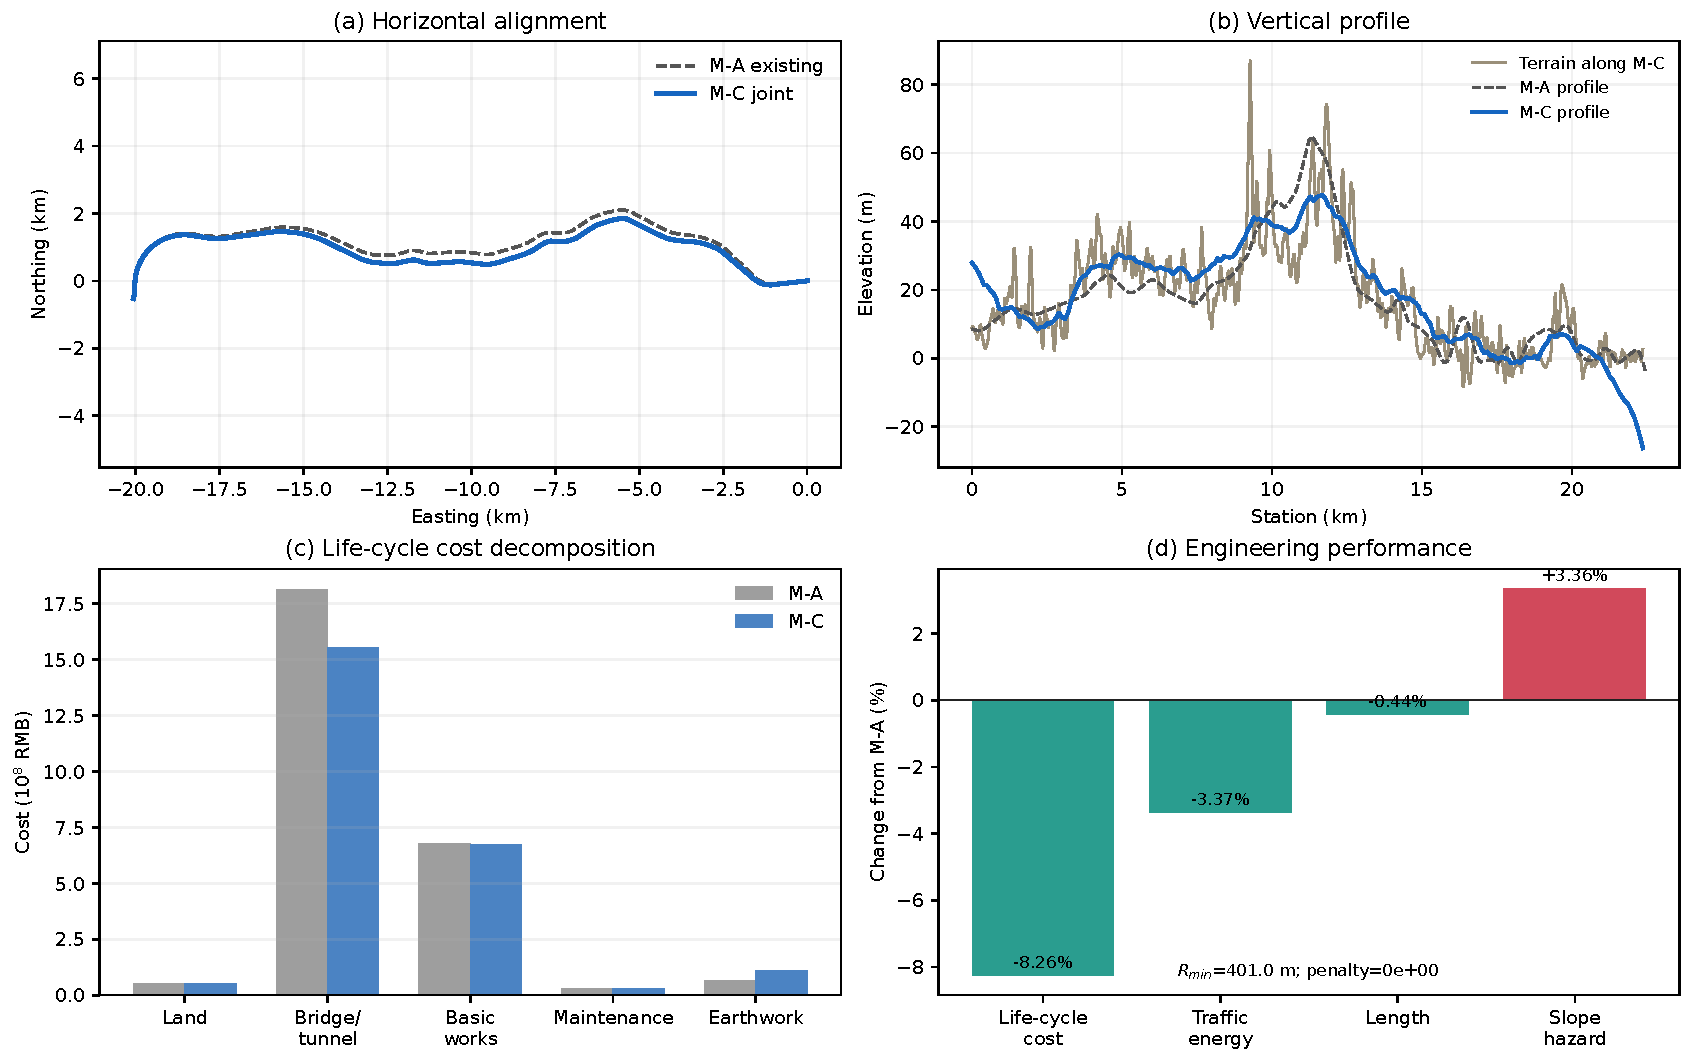
\includegraphics[width=\textwidth]{c132_scheme_summary.pdf}
\caption{Pinned M-A/M-C comparison: plan, profile, cost decomposition and headline changes. The unanchored terminal profile is shown rather than concealed.}
\label{fig:scheme}
\end{figure}

The cost mechanism is dominated by structure substitution. Bridge/tunnel cost decreases by 261.4 million RMB, whereas earthwork cost increases by 45.5 million RMB; maintenance rises by 0.88 million RMB, yielding a net cost reduction of 218.2 million RMB. Land and basic works also decrease slightly. Hence the saving is not attributable only to route shortening; it reflects a larger reduction in structures offset by greater earthwork.

The cost--energy sweep contains 21 weighted searches. Figure~\ref{fig:pareto} shows the feasible points and the entropy-selected M-C. The feasibility and 10\% budget gates remove inadmissible or structure-heavy endpoints before the final entropy score is evaluated.

\begin{figure}[t]
\centering
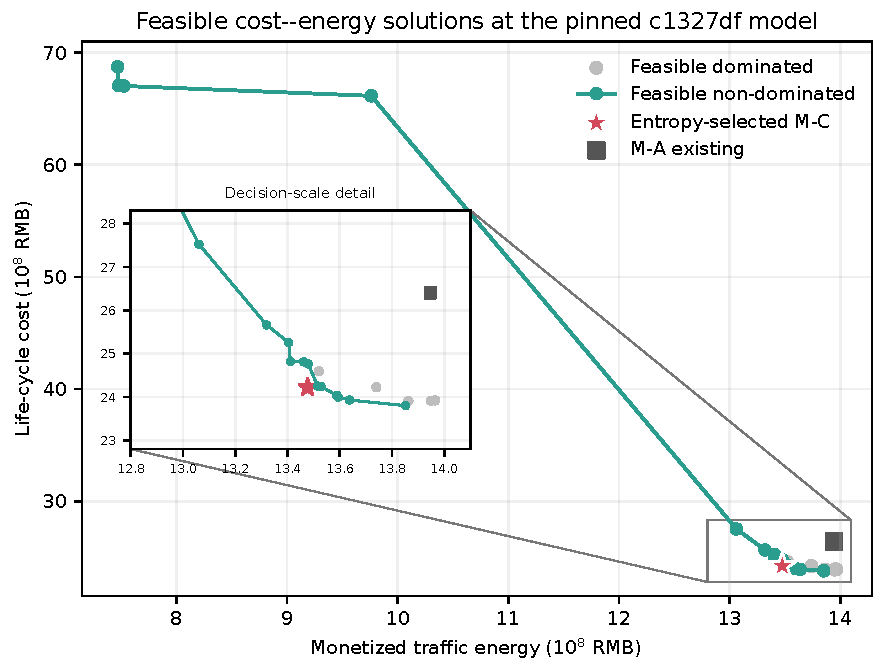
\includegraphics[width=\linewidth]{c132_pareto.pdf}
\caption{Feasible cost--energy solutions and the entropy-selected compromise in the pinned model.}
\label{fig:pareto}
\end{figure}

\subsection{Joint versus sequential optimization}

The sequential control achieves lower raw values than the joint solution, but it violates the minimum-radius requirement. Table~\ref{tab:sequential} therefore distinguishes numerical objective values from admissible engineering performance. Freezing the plan after stage one leaves the profile stage unable to repair the 397.06-m plan radius; its penalty remains 0.07359. The feasible M-C is the preferred result despite its higher raw cost and energy.

\begin{table}[t]
\centering
\caption{Joint and two-stage results under common objective references.}
\label{tab:sequential}
\begin{tabular}{lrrr}
\toprule
Metric & M-A & Two-stage & Joint M-C \\
\midrule
Cost ($10^8$ RMB) & 26.4061 & 23.1582 & 24.2239 \\
Energy ($10^8$ RMB) & 13.9460 & 13.4569 & 13.4766 \\
Length (km) & 22.4618 & 22.3659 & 22.3635 \\
$R_{min}$ (m) & 422.43 & 397.06 & 401.03 \\
Penalty & 0 & 0.07359 & 0 \\
Decision status & feasible & infeasible & feasible \\
\bottomrule
\end{tabular}
\end{table}

\subsection{IJS mechanism ablation}\label{sec:ablation}

At 500 generations, complete IJS has the lowest observed mean scalar objective, 0.6808 versus 0.9133 for JS, an observed gap of 25.45\% (Table~\ref{tab:ablation}). Among the single-operator variants, JS+DE has the largest observed same-generation gap from JS; Tent alone has a small, statistically inconclusive gap in the unadjusted rank-sum test. IJS reaches the final JS level at generation 187 in the stored convergence record. However, the full method also uses about three times as many objective evaluations per generation. The table therefore demonstrates same-generation performance only.

\begin{table}[t]
\centering
\caption{Thirty-run profile-testbed ablation. $p$ values are unadjusted independent-sample rank-sum tests; NFE differs by variant.}
\label{tab:ablation}
\begin{tabular}{lrrrrr}
\toprule
Variant & Mean $F$ & SD & $F_{100}$ & Gap from JS & $p$ \\
\midrule
JS & 0.9133 & 0.0637 & 2.547 & -- & -- \\
JS+Tent & 0.8989 & 0.0605 & 2.227 & 1.58\% & 0.464 \\
JS+L\'evy & 0.8787 & 0.0558 & 2.095 & 3.79\% & 0.0555 \\
JS+DE & 0.6926 & 0.0315 & 1.679 & 24.17\% & $3.02\times10^{-11}$ \\
IJS & \textbf{0.6808} & 0.0340 & \textbf{1.292} & \textbf{25.45\%} & $3.02\times10^{-11}$ \\
\bottomrule
\end{tabular}
\end{table}

\subsection{Multi-algorithm comparison}

IJS has the lowest recorded mean $F$ at all six resolutions (Table~\ref{tab:benchmark}). At PJ6, IJS and JS return feasible solutions in all ten runs, whereas the four other methods return penalty-dominated solutions. IJS takes about 1.9 times the wall time of JS at PJ1--PJ5 and about 2.8 times at PJ6, while also performing more objective calls. The defensible conclusion is therefore that the implemented multi-phase search attains the lowest observed same-generation objective and stronger high-resolution feasibility in this record, not that it is superior under equal computational budget.

\begin{table*}[t]
\centering
\caption{Objective mean (SD) over ten runs. Equal generations do not imply equal NFE.}
\label{tab:benchmark}
\scriptsize
\resizebox{\textwidth}{!}{\begin{tabular}{lrrrrrr}
\toprule
Algorithm & PJ1 (95) & PJ2 & PJ3 & PJ4 & PJ5 & PJ6 (500) \\
\midrule
IJS & \textbf{.6617 (.0051)} & \textbf{.5986 (.0045)} & \textbf{.7087 (.0045)} & \textbf{.7090 (.0033)} & \textbf{.7778 (.0078)} & \textbf{.8333 (.0019)} \\
JS & .6771 (.0052) & .6104 (.0049) & .7237 (.0063) & .7215 (.0066) & .7954 (.0020) & .8563 (.0060) \\
NSGA-II & .6792 (.0045) & .6240 (.0057) & .7282 (.0053) & .7287 (.0080) & .8104 (.0084) & 12.8859 (.7330) \\
GA & .7103 (.0088) & .6478 (.0171) & .7515 (.0090) & .7489 (.0071) & 5.3906 (.5481) & 25.6024 (1.0630) \\
PSO & .7023 (.0116) & .6370 (.0113) & .7436 (.0070) & .7632 (.0072) & 9.1988 (.9109) & 32.7437 (.6336) \\
GWO & .6843 (.0065) & .6194 (.0070) & .7233 (.0046) & .7276 (.0070) & 1.1104 (.0158) & 3.2157 (1.5706) \\
\bottomrule
\end{tabular}}
\end{table*}

\subsection{Sensitivity within the pinned model family}

All 237 stored sensitivity re-optimizations are marked feasible under their implemented checks. Traffic growth dominates the monetary energy response; cost is less responsive to demand, fleet and energy-price factors because most infrastructure expenditure occurs at construction. Higher EV penetration moderates the high-demand energy burden, whereas combined fuel and electricity price growth raises $E$.

The spectral-width response is strong and then saturating: optimized $C$ decreases from 2.568 billion RMB at $W=200$ m to 2.239 billion RMB at $W=2{,}500$ m. The result supports the interpretation of $W$ as search flexibility, not a hard corridor width. Changing $E_{ext}$ from 50 to 75 and 100 m shifts $C$ to 2.281, 2.355 and 2.474 billion RMB, while $E$ stays near 1.355 billion RMB. These values show that bridge assumptions materially affect economic results.

\begin{figure}[!htbp]
\centering
\begin{subfigure}{.78\textwidth}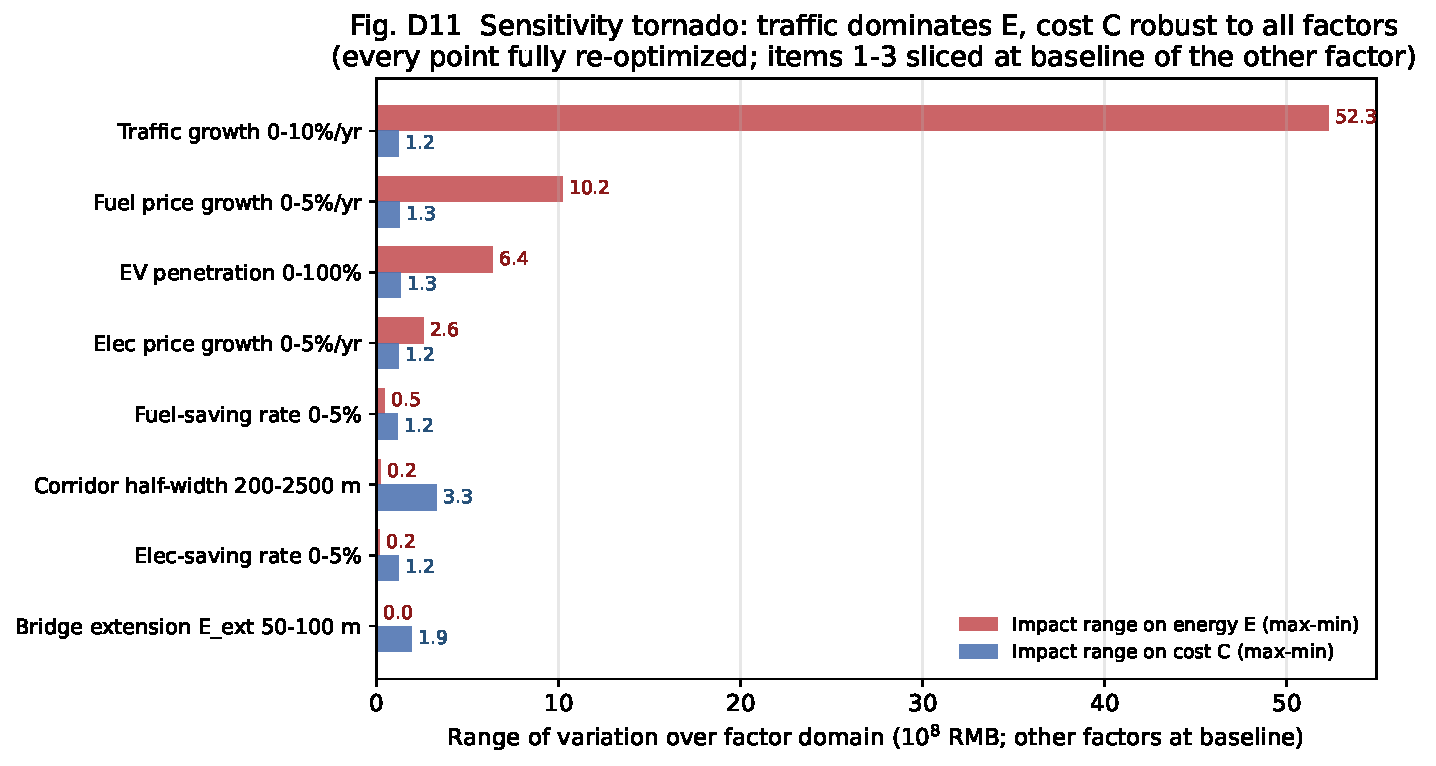
\includegraphics[width=\linewidth]{sensitivity_tornado.pdf}\caption{Relative importance of operating scenarios.}\end{subfigure}\\[3mm]
\begin{subfigure}{.78\textwidth}
\includegraphics[width=\linewidth]{corridor_sensitivity.pdf}\caption{Re-optimization over spectral width $W$.}\end{subfigure}
\caption{Sensitivity results already present at the pinned commit.}
\label{fig:sensitivity}
\end{figure}
\FloatBarrier

\section{Discussion}

\subsection{Engineering interpretation}

The 8.26\% and 3.37\% reductions are case-specific, model-based changes under common quantities and unit rates. Their value lies in the traceable mechanism. M-C is 0.44\% shorter, but the 261.4-million-RMB structure reduction is much larger than the cost implied by 98.3 m of length alone. The optimizer trades more earthwork and a slightly higher slope-hazard diagnostic for lower structure exposure and operating energy.

The sequential comparison reinforces the priority of feasibility. Its lower raw objectives cannot be interpreted as a better design because $R_{min}=397.06$ m violates the 400-m threshold. Collaborative search retains the ability to change plan and profile together near a constraint boundary; the pinned record shows a feasible joint alternative where the particular sequential run is infeasible.

\subsection{Role of spatial data and IJS}

Candidate-specific DEM sampling changes the objective landscape because lateral movement changes ground elevation rather than only distance. OSM intersections convert location into bridge demand, while the connected mountain mask makes ecological-tunnel length endogenous. These mechanisms improve auditability but remain planning abstractions: OSM lacks reliable deck elevations and parcel attributes, and the reconstructed DEM is not a survey-grade pre-construction surface.

Tent, L\'evy and DE play plausible coverage, exploration and refinement roles. Among the single-operator variants, JS+DE has the largest observed same-generation gap from JS; this observation does not isolate an evaluation-budget-normalized DE effect. The algorithm evidence therefore supports the implemented workflow and generates an equal-NFE research hypothesis; it does not isolate an intrinsic 25.45\% advantage.

\subsection{Limitations and validity boundary}\label{sec:limitations}

\begin{enumerate}[leftmargin=*,label=(\arabic*)]
\item The vertical start and end elevations are free. In the selected M-C, the terminal elevation is visibly below the existing endpoint. This can affect both earthwork and one-direction energy; the 8.26\%/3.37\% result must not be presented as a fixed-tie-in design.
\item Energy is evaluated for one representative direction. A bidirectional, direction-weighted model with calibrated regenerative braking is required to remove net-elevation sensitivity.
\item Adjacent grade change is only a proxy for vertical-curve design. Explicit crest/sag radii, curve lengths, sight distance, clothoid/arc segmentation and full plan--profile coordination checks are absent.
\item The quasi-natural DEM is reconstructed from a built-road surface at about 8.8-m resolution. OSM coverage and crossing classifications are heterogeneous, and obstacle vertical clearances are not verified.
\item Building density does not enter this pinned model. Urban avoidance shown in conceptual graphics must not be interpreted as a computed constraint or benefit.
\item Cost rates are planning estimates. Geology, hydrology, parcel acquisition, resettlement, construction staging, embodied carbon and uncertainty require project-specific data.
\item The engineering solution is one optimization run. Ablation and benchmarks use same generations but unequal NFE; their rank-sum tests are unadjusted. Algorithm superiority therefore remains unconfirmed under equal budget.
\end{enumerate}

Accordingly, the framework provides auditable corridor-planning evidence and a reproducible computational case. It does not replace detailed geometric design or support a universal saving rate.

\section{Conclusions}

This study links candidate three-dimensional highway geometry to quasi-natural terrain, OSM-triggered structures, life-cycle cost and mixed fuel--electric traffic energy. A 275-variable collaborative representation is searched by IJS, and feasibility, budget and non-dominance precede entropy-based compromise selection.

At the pinned \texttt{c1327df} version, the feasible Guangzhou North Ring joint solution reduces cost by 8.26\% and monetized energy by 3.37\%, shortens the line by 0.44\%, and satisfies the radius requirement with $R_{min}=401.03$ m and zero penalty. The principal economic mechanism is a 261.4-million-RMB structure reduction that exceeds the 45.5-million-RMB earthwork increase. A lower-objective two-stage result is rejected because its radius is 397.06 m. IJS has the lowest observed same-generation objective in the stored ablation and benchmark, but unequal NFE prevents an equal-budget superiority claim.

The most important next methodological correction is to anchor both vertical endpoints and evaluate bidirectional traffic before treating the alignment as design-grade. Equal-NFE multi-seed algorithm comparison, explicit vertical curves and survey/parcel data are also needed. These are limitations and future work, not supplementary experiments used to alter the results reported here.

\section*{Data and code availability}
All manuscript numbers and manuscript-only figures are tied to Git commit \texttt{c1327df}; its full hash is stored in the source manifest. The draft package contains a source-value snapshot, SHA-256 manifest and a figure script that reads the immutable Git objects without executing an optimizer. GNSS and project-derived data may be subject to owner restrictions. A public repository DOI should be added after anonymization review.

\section*{CRediT authorship contribution statement}
\textbf{[Author placeholders]}: Conceptualization, Methodology, Software, Validation, Investigation, Data curation, Visualization, Writing---original draft, Writing---review \& editing. Replace with verified author roles before submission.

\section*{Declaration of competing interest}
The authors declare that they have no known competing financial interests or personal relationships that could have appeared to influence the work reported in this paper. Confirm this statement with all authors before submission.

\section*{Acknowledgements}
Funding agency, grant number and non-author contributions are anonymized and must be completed before submission.

\bibliographystyle{elsarticle-num}
\bibliography{../references}

\end{document}
